 % -*- coding: utf-8 -*-
\documentclass[conference]{IEEEtran}
\IEEEoverridecommandlockouts
% The preceding line is only needed to identify funding in the first footnote. If that is unneeded, please comment it out.
\usepackage{cite}
\usepackage{amsmath,amssymb,amsfonts}
\usepackage{algorithmic}
\usepackage{graphicx}
\usepackage{textcomp}
\usepackage{xcolor}
\usepackage[varg]{txfonts}%%!!
\usepackage{url}

\def\BibTeX{{\rm B\kern-.05em{\sc i\kern-.025em b}\kern-.08em
    T\kern-.1667em\lower.7ex\hbox{E}\kern-.125emX}}
\begin{document}

\title{Magnet or Sticky? A Stack Overflow Tag-by-Tag Typology\\
% {\footnotesize \textsuperscript{*}Note: Sub-titles are not captured in Xplore and
% should not be used}
% \thanks{Identify applicable funding agency here. If none, delete this.}
}
\author{\IEEEauthorblockN{1\textsuperscript{st} Kotori Hieda}
\IEEEauthorblockA{\textit{Information Science and Electrical} \\
\textit{Engineering. Kyushu University}\\ 
Fukuoka, Japan \\
hieda@f.ait.kyushu-u.ac.jp}
\and
\IEEEauthorblockN{2\textsuperscript{nd} Yu Mingzhe}
\IEEEauthorblockA{\textit{Information Science and Electrical} \\
\textit{Engineering. Kyushu University}\\ 
Fukuoka, Japan \\
yumingzhe@f.ait.kyushu-u.ac.jp}
\and
\IEEEauthorblockN{3\textsuperscript{rd} Olivier Nourry}
\IEEEauthorblockA{\textit{Information Science and Electrical} \\
\textit{Engineering. Kysushu University}\\ 
Fukuoka, Japan \\
onourry3@gmail.com}
\and
\IEEEauthorblockN{4\textsuperscript{th} Yasutaka Kamei}
\IEEEauthorblockA{\textit{Faculty of Information Science and} \\
\textit{Electrical Engineering. Kyushu University}\\
Fukuoka, Japan \\
kamei@ait.kyushu-u.ac.jp}
% \and
% \IEEEauthorblockN{4\textsuperscript{th} Given Name Surname}
% \IEEEauthorblockA{\textit{dept. name of organization (of Aff.)} \\
% \textit{name of organization (of Aff.)}\\
% City, Country \\
% email address or ORCID}
% \and
% \IEEEauthorblockN{5\textsuperscript{th} Given Name Surname}
% \IEEEauthorblockA{\textit{dept. name of organization (of Aff.)} \\
% \textit{name of organization (of Aff.)}\\
% City, Country \\
% email address or ORCID}
% \and
% \IEEEauthorblockN{6\textsuperscript{th} Given Name Surname}
% \IEEEauthorblockA{\textit{dept. name of organization (of Aff.)} \\
% \textit{name of organization (of Aff.)}\\
% City, Country \\
% email address or ORCID}
}

\maketitle

\begin{abstract}
Stack Overflow (SO) is one of the most popular question and answer sites for software developers. SO stores posts assigned with tags that correspond to the keywords of each question. If a developer asks a question related to Python and tags a post with the ``Python'' tag, developers interested in Python can easily find the post. Since 2008, SO has become one of the most trusted online communities. In this study, we explore developers' interest by analyzing how they use tags. We classify tags using the following metrics: (1) attractive, (2) fluctuating, (3) stagnant, and (4) terminal based on magnet values and sticky values. We analyze the data of table ``Posts'' which consists of approximately 42 million SO posts and the data of table ``Users'' which contains approximately 9 million rows of user information. Results reveal that: (1) There is a relationship between the magnetic and sticky values of a tag and the evolution of a project related to said tag, i.e., the creation of new software or the termination of the project. (2) The characteristics of the classified tags do not change much.
\end{abstract}

\begin{IEEEkeywords}
magnet, sticky, tag, user migration, OSS census
\end{IEEEkeywords}

% 1
\section{Introduction}
The Pew Research Center (PRC)~\cite{communityeconomic} is the U.S. fact finder that provides information on social problems and demographic trends that shape the United States and the world.  
\emph{Magnet states} are defined as states where a high percentage of the population migrated from other states and \emph{sticky states} are states where a high percentage of adults have been living in that same state since birth. 
Nevada is a \emph{magnet states} because  86\% of the population migrated from other states. It is possible to find the movement of American citizens by studying this demographic trend.

For software developers, understanding other developers' interests are important as the popularity of developers have advantages. Many developers like to work with convenient and easy-to-use tools. To develop a project efficiently, a project needs to attract good developers over a long period of time.

In this study, we focus on new and existing topics of Stack Overflow (SO). Inspired by previous studies~\cite{yamashita2016magnet}, we apply the magnet and the sticky metrics to the topics collected in SO. 
The magnet metric is the number of existing developers who remain involved with a specific topic.
We examined magnet and sticky values of tags by classifying them using one of three categories: \emph{programming language}, \emph{framework}, and \emph{environment}. We also look at the evolution of multiple software and web services companies. If any change or evolution is discovered, we investigate whether there is a relationship between change or evolution and magnet and sticky values.

We address the following two research questions:

\noindent \textbf{(RQ1) What are the magnet and sticky values of popular SO tags?}\par
We find that in many cases, the sticky value is higher than the magnet value. In addition, the decrease rate was higher for the magnet value than it was for the sticky value.

\noindent \textbf{(RQ2) How do magnet and sticky values change over time?}\par
When the status of a tag changes in four types, there may have been some change or evolution in that tag or another tag related to that tag.
\section{Definition of Magnet and Sticky} \label{magnet}
This section describes how we measure the appeal and adhesion of users on different topics. Following the Pew Research Center (PRC) definition~\cite{communityeconomic}, we use the magnet and sticky metrics to illustrate the migratory trends of U.S. citizens. The PRC defines magnet states as states where a large proportion of adults are from other states and defines sticky states as state where a high share of the adults who were born there live there now. These definitions are for population studies where a single adult can only live in one state at a time, however, so these definitions are inapplicable to the topics discussed by the SO users as users can ask or answer questions on several topics at the same time. Therefore, we redefined magnet and sticky so that they can be applied in SO. 

\noindent
\textbf{Magnet.} Magnet topics attract a large proportion of new users; thus, the magnet value is calculated as the percentage of new users who ask or answer questions during a year.

\noindent
\textbf{Sticky.} In sticky topics, users continue to participate in the same topic. Thus, we calculate the stickiness of a topic as the proportion of users who remain involved in the topic’s discussion over the years.


\subsection*{\textit{\textbf{Magnet and Sticky in SO}}}

SO content is made of user comments, questions and answers~\cite{liu2018mining} called Posts in the  SOTorrent\cite{baltes2018sotorrent} database. Each question has one or more tags that separate the question into different topics. Each post has an author, a participant and a question. We defined who is the participant of which topic as follows. For example, user A answers a question with a Java tag, user B answers with an Apache tag, and user C answers with a Linux tag. At this time, User C is a participant in Java, Apache, and Linux topics.


\noindent
\textbf{Example (Calculating magnet and sticky values).}
To calculate magnet and sticky values of topics that belong to a major category, we use a total of three questions (α,β,γ) and five users (A, B, C, D, E). Users A, B and C registered in 2017 and users D and E register in 2018~\cite{yamashita2016magnet} as shown in Figure~\ref{fig:example1}.
% To calculate magnet and sticky values of topics that belong to a major category, we use a total of six questions (a, b, c, d, e, f) and seven users (A, B, C, D, E, F, G); the Last Activity Date of question a, b, c was in 2017, and question d, e, f in 2018. The registration date of user A, B, C, D was in 2017, and the registration date of user E, F, G was in 2018~\cite{yamashita2016magnet} as shown in Figure ~\ref{fig:example1}.

\begin{figure}[t]
 \centering
 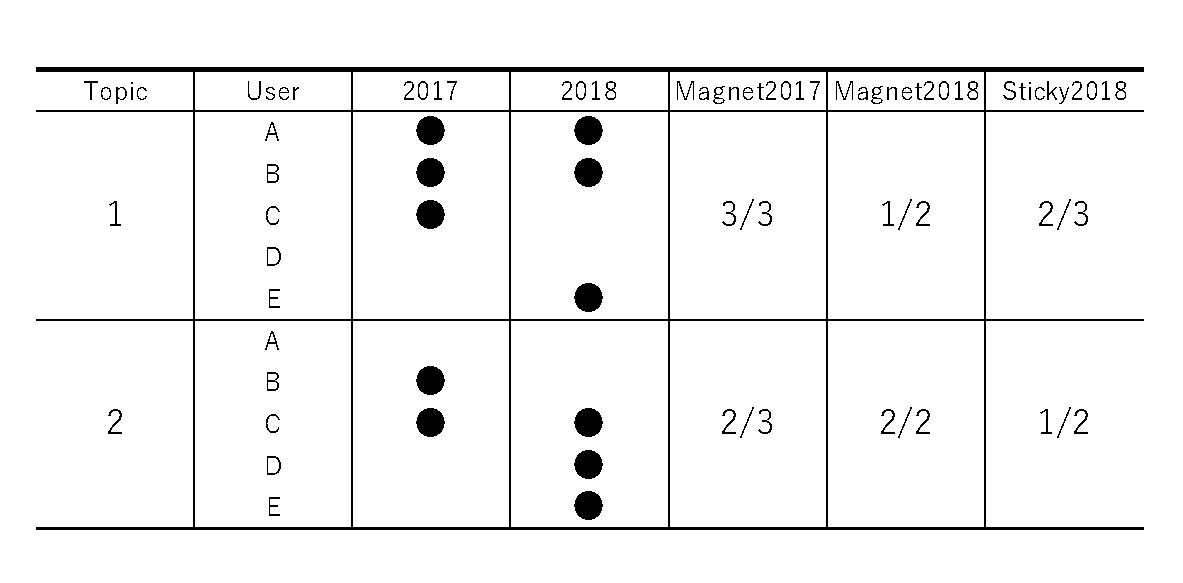
\includegraphics[width=1.0\hsize]{img/fig11.eps}  
 \caption{Example of magnet and sticky values definition} 
 \label{fig:example1} 
\end{figure}

Filled black circles in Figure~\ref{fig:example1} represent user activities (e.g., creating questions, answering questions, and adding comments to the questions) in a topic during specific period.
 % For example, while User A has activities in Topic 1 of the years 2017 and 2018, but he/she has no activities in Topic 2.

To calculate the magnet metric, we observe three new users who registered their account in 2017 (A, B, C), who registered their account in 2017 and participate in topic 1 and two users (B, C) who participate in topic 2. In 2017, the magnet value of topic 1 was 3/3 and the magnet value of topic 2 was 2/3.
% To calculate the magnet metric, we observe four new users who registered their accounts in 2017 (A, B, C, and D), and all of them discuss topic 1, whereas two of them (B, C) participate in the discussion topic 2 and 3. In this case, the Magnet value of topic 1 in 2017 is 4/4, topic 2 is 2/4, and topic 3 is 2/4.

To calculate the sticky metric of topic 1, three users participated in the discussion in 2017 (A, B, and C). Only two of them participated in the discussion in 2018 (A, B). Hence, the sticky value of project 1 is 2/3. In 2017, two users took part in the discussion for topic 2 (B and C); however, only one of them participated in the discussion in 2018 (C). Though new users D and F participated in the discussion in 2018, we still calculate the value of sticky as 1/2.
% To calculate the sticky metric on topic 1, three users participated in the discussion in 2017 (A, B, and C). Only one of them participated in the discussion in 2018 (A). Hence, the sticky value of project 1 is 1/4. In topic 2, two users participated in the discussion in 2017 (B and C); however, only one of them participated in the discussion in 2018 (B). Though new users E, F, G, participated in the discussion in 2018, we still calculate the value of sticky as 1/2. For the same reason, the sticky of topic 3 is 2/2 in 2018.\\

\noindent
\textbf{Example (Merging similar subjects into one topic).}
We merge subjects (i.e., tags) that belong to analogous subjects into one topic. We consider different version numbers (e.g., tag ``Python-2.7'' and tag ``Python-3.6'') as one of the common examples of analogous tags. 
% We merge subjects (i.e., tags) that belong to analogous subjects into one topic. For example, we consider that different version numbers (e.g., tag ``Python-2.7'' and tag ``Python-3.6'') are one of the common examples of analogous tags. 

\begin{figure}[t]
 \centering
 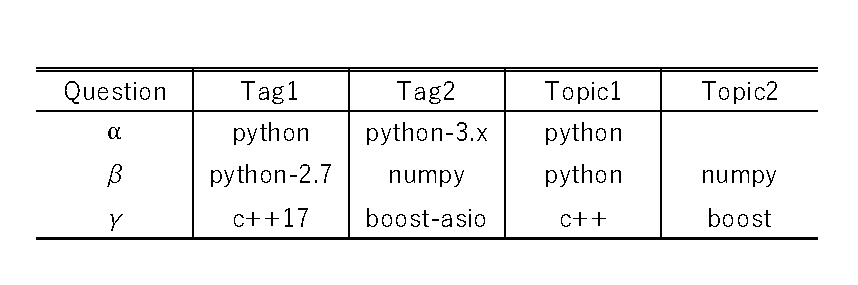
\includegraphics[width=1.0\hsize]{img/ff2.eps}  
 \caption{Example of a merge of tags belonging to analogous subjects} 
 \label{fig:example2} 
\end{figure}

We consider all different versions of a tool, as well as derived tools, to belong to the same topic. For example, the tag ``reactjs,'' ``react-router,'' ``reactjs-flux,'' ``create-react-app'' should be merged into one topic ``react.'' We can get this information from the “Related Tag” column of the ``Tag Info of SO.''
% We also need to merge derivatives of the same technology on different platforms, merge derivatives of special tools in a certain tool family, or a combination of technology with a common used library, etc. For example, the tag ``reactjs,'' ``react-router,'' ``reactjs-flux,'' ``create-react-app'' should be merged into one topic ``react.''
% Of course, the difference in version number is the most common example of analogous tags. The rest of examples includes derivatives of the technology on different platforms, commonly used libraries, or specific tools in a tool family, etc. for example topic ``react'' includes tag ``reactjs'', ``react-router'', ``reactjs-flux'', ``create-react-app'' etc. 
% We can get this information from the ``Related Tag'' column of the ``Tag Info of SO.''

Figure~\ref{fig:example2} shows that question α has tags ``python'' and ``python-3.x'' and question β has the tag ``python-2.7.'' According to our merge rule, they all belong to topic ``python.'' The question γ has the tag ``c++17,'' showing that it belongs to topic ``c++.'' Therefore, question β also belongs to topic ``numpy'' and question γ also belongs to topic ``boost.''
% Figure~\ref{fig:example2} shows that question a has tag 1.0, question b has tag 1.1, and question f has tag 1.2. According to our merge rule, they all belong to topic 1. The question c has tag 2.0 and tag 3.1, showing that it belongs to topic 2 and 3. Therefore, question d belongs to topic 2, and question e belongs to topic 3.


\begin{figure*}[t]
 \centering
 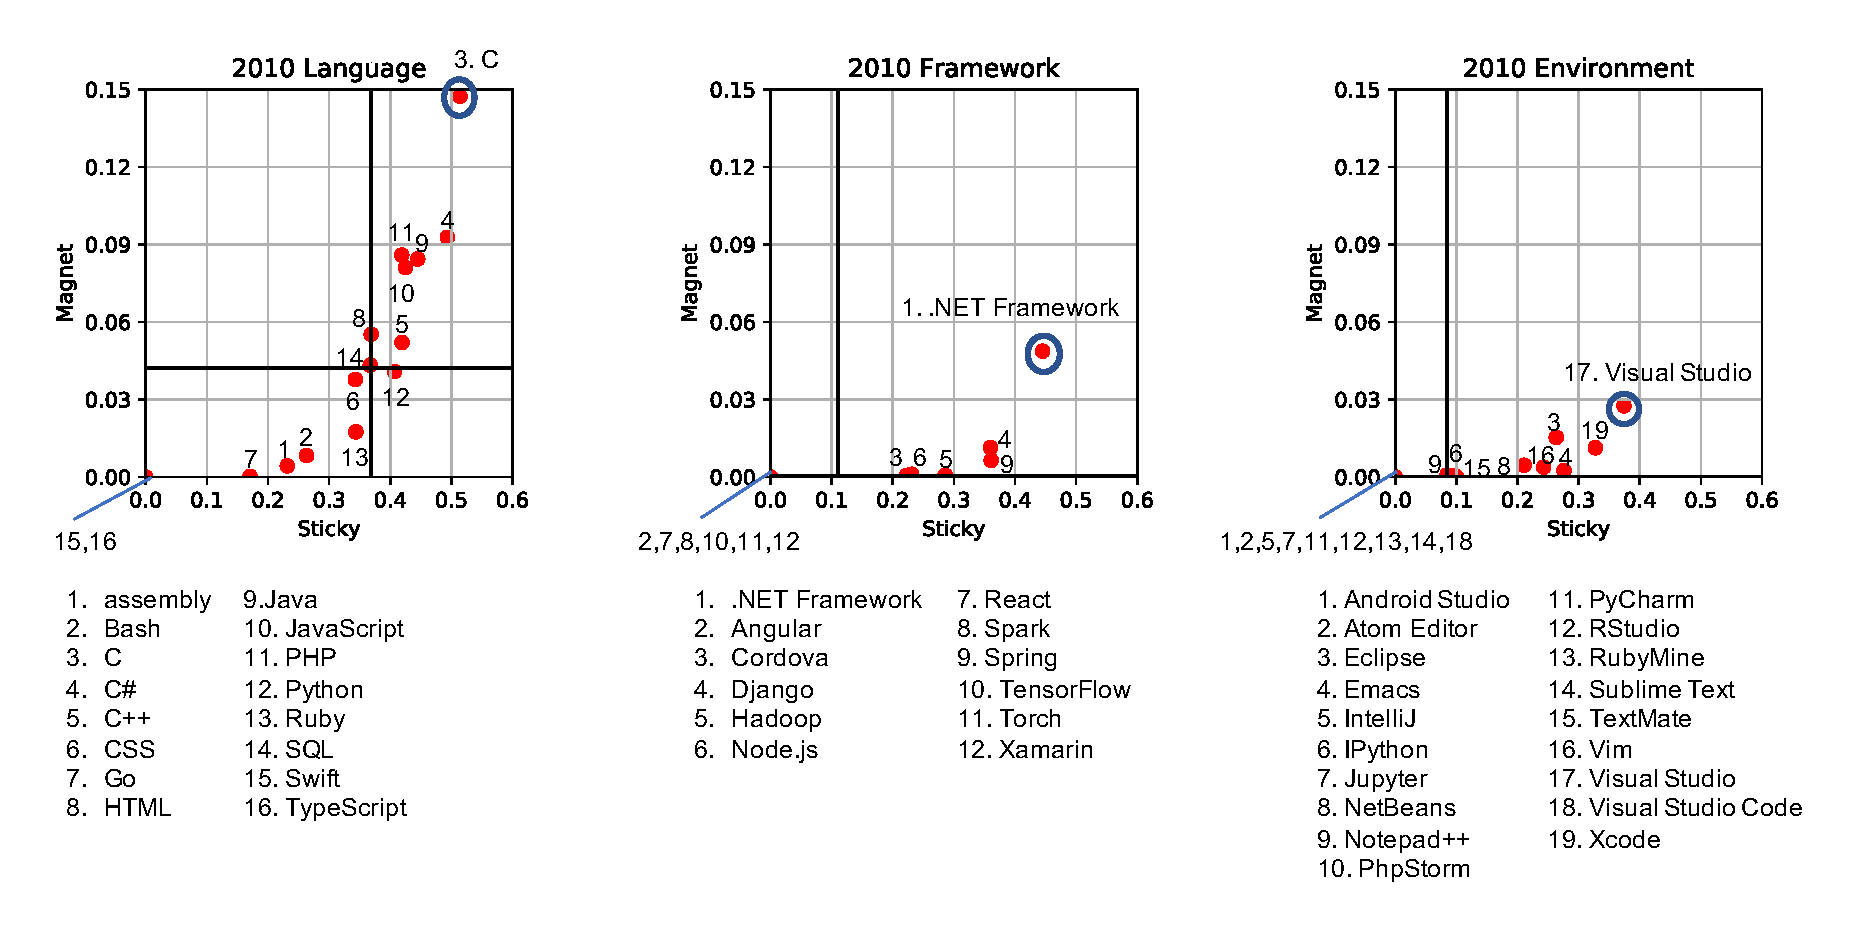
\includegraphics[width=1.0\hsize]{img/2010allnew.eps}  
 \caption{Distribution of Magnet and Sticky values in Programing Language, Framework and Environment} 
 \label{fig:2010} 
\end{figure*}


\section{Dataset}
We analyze the SO dataset (SOTorrent) provided by Sebastian Baltes et al.~\cite{msr2019challenge}. SOTorrent is an open dataset based on the official SO data dump. SOTorrent provides access to the version history of SO content at the level of whole posts and individual text and code blocks. It connects code snippets from SO posts to other platforms by aggregating URLs from surrounding text blocks and comments, and by collecting references from GitHub files to SO posts.

The dataset consists of 20 different data tables.
However, we analyze the data of table \emph{Posts} which consists of approximately 42 million posts from SO and table \emph{Users} which contains approximately 9 million rows of User information from July 2008 to September 2018. For the purpose of this study, we looked at the users, tags and the date each question was posted in order to calculate magnet and sticky value. Moreover, we only considered users who ask or answer questions in SO. Those who only comment or like/dislike questions and answers were excluded to narrow down those who are really interested in the topic.

\begin{table}[t]
 \centering
 \caption{Average Quadrant Transition rate}
 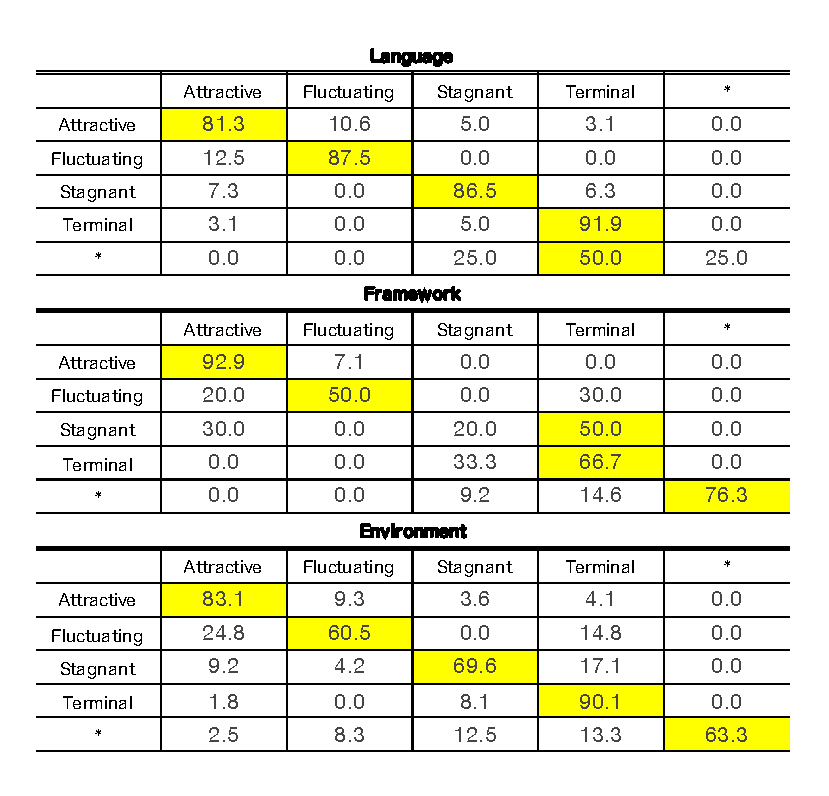
\includegraphics[width=1.0\hsize]{img/transitionnew.eps} 
 \label{table2} 
\end{table}

\begin{table*}[t]
 \centering
 \caption{Quadrant Transition of Framework 2010 - 2018} 
 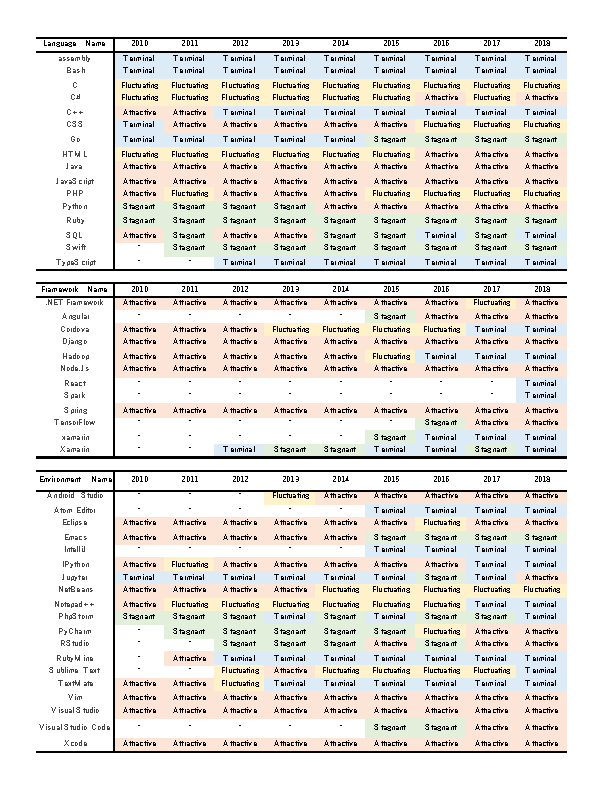
\includegraphics[width=1.0\hsize]{img/AFSTnew.eps} 
 \label{table1} 
\end{table*}


\section{Study Results} %paragraph4
In this section, we provide answers to the following questions:
\subsection{(RQ1) What are the magnet and sticky value of popular SO tags?}

\noindent
\textbf{Approach.}
We calculated magnet and sticky values as defined in Section~\ref{magnet}. We plot the magnet value on the vertical axis and the sticky value on the horizontal axis. We classify the plotted points into four quadrants.\\
\textbf{Attractive:} Tags with a high magnet and sticky value. By understanding the tags, we can discover the interests of developers.\\
\textbf{Fluctuating:} Tags with a high magnet and low sticky value. This tag attracts people but only for a short period of time. Developers lose interests over time.\\
\textbf{Stagnant:} Tags with a low magnet and high sticky value. This tag does not attract many new users, but it can retain existing users.\\
\textbf{Terminal:} Tags with low magnet and sticky value. This tag can neither attract new developers nor keep them interested.

The median of the magnet and sticky values for each year is used for the quadrant threshold because the median is unaffected by outliers. From the sticky value definition in Section~\ref{magnet}, the sticky value depends on the number of users that remain involved in a tag’s discussion over time. To answer RQ1, we calculated the sticky value for nine years from 2009 to 2018. We used information posted by users only those who posted questions or answers with tags in SO.
 The magnet and sticky values depend on the number of new tag users, but, if the number of new tag users in a year is too low, the values will be too small to accurately classify tag status as attractive, fluctuating, stagnant, and terminal. To remove noise, we set thresholds for each topic. If the magnet and sticky values are less than the threshold, we assign an asterisk to its magnet and sticky value.

We did not analyze all the tags at once, but divided them into three categories for analysis. The selected categories and their contents are:
\begin{itemize}
\item programming languages ​​(assembly, Bash, C, C♯, C ++, CSS, Go, HTML, Java, JavaScript, PHP, Python, Ruby, SQL, Swift, TypeScript)
\item frameworks ( .NET Framework, Angular, Cordova, Django, Hadoop, Node.js, React, Spark, Spring, TensorFlow, Torch, Xamarin)
\item environment (Android Studio, Atom Editor, Eclipse, Emacs, IntelliJ, IPython, Jupyter, NetBeans, Notepad++, PhpStorm, PyCharm, RStudio, RubyMine, Sublime Text, TextMate, Vim, Visual Studio, Visual Studio Code, Xcode)
\end{itemize}

We chose these tags based on SO's survey of over 100,000 developers in 2018~\footnote{\url{https://insights.stackoverflow.com/survey/2018}}. We focused on tags used by more than 5\% of developers who answered the questionnaire. 

%The year when StackOverflow released these data is May 2008. Since the sticky value is calculated from the difference between the previous year and the current year, the distribution chart of magnet and sticky value according to three categories in 2010 is shown as the first year for which yearly data of sticky value can be obtained.

% 我々は全てのタグを一度に調査するのではなく3つのカテゴリに分けて分析をした。その方が特徴を見つけやすいからである。我々が選んだカテゴリたちとその内容はプログラミング言語(assembly, Bash, C, C♯, C++, CSS, Go, HTML, Java, JavaScript, PHP, Python, Ruby, SQL, Swift, TypeScript), フレームワーク(.NET Framework, Angular, Cordova, Django, Hadoop, Node.js, React, Spark, Spring, TensorFlow, Torch, Xamarin),そして環境(Android Studio, Atom Editor, Eclipse, Emacs, IntelliJ, IPython, Jupyter, NetBeans, Notepad++, PhpStorm, PyCharm, RStudio, RubyMine, Sublime Text, TextMate, Vim, Visual Studio, Visual Studio Code, Xcode)である。
% これらを選んだ理由は2018年にStack Overflowが10万人を超える開発者たちにとったアンケートの結果に基づいている。Stack Overflowは開発者たちに使用するタグたちについてのアンケートをとり、我々はアンケートに答えた開発者たちの5\%以上が使用しているタグたちに絞って調査した。StackOverflowがこれらのデータを公開した年は2008年5月である。sticky値は前年と当年の差から算出しているため、sticky valueの通年データが取れる最初の年として2010年の3カテゴリ別のmagnetとsticky valueの分布図を示す。

% The categories we selected and their contents are programming languages (assembly, Bash, C, C\#, C++, CSS, Go, HTML, Java, JavaScript, PHP, Python, Ruby, SQL, Swift, TypeScript), framework (.NET, Angular, Cordova, Django, Hadoop, Node.js, React, Spark, Spring, TensorFlow, Torch, Xamarin), and the environment (Android Studio, Atom Editor, Eclipse, Emacs, IntelliJ, IPython, Jupyter, NetBeans, Notepad++, PhpStorm, PyCharm, RStudio, RubyMine, Sublime Text, TextMate, Vim, Visual Studio, Visual Studio Code, Xcode) because these three categories are one of the most popular tag categories used in stack overflow. We also analyzed by picking the top tags that are popular among each category. Tags that are not popular have no character and we do not know anything from that. By dividing it for each category, it became easier to see the features. We show distribution map of magnet and sticky value by 3 categories of 2010 as one of the characteristics easy to understand.

%\textbf{Manual analysis:}
%Figure~\ref{fig:2010} shows the distribution of magnet and sticky values in programing language, framework, and environment (2010)\footnote{We choose the year 2010 because it is the first year for which yearly data of sticky value can be obtained.}. 
% We find that .NET Framework is a high magnet and sticky value. 

%.NET framework 

%Beginner developers can relatively easily develop advanced software using . Are there many reasons why the .NET Framework's sticky value is high reasons most conveniently? It is the foundation system for building applications. 

%Java has long been popular and attractive as it is one of the most famous programming languages ​​in the world. Eclipse especially attracted people in 2010, so the magnet value is high.

% 図~\ref{plotframe2010}の2009 Frameworkにおいて、.NET Frameworkは高いマグネットとスティッキー値である。高いマグネットとスティッキー値であることは非常に良いと言える。.NET Framework は、2006年11月にマイクロソフトに発表された。これはネットワーク上でアプリケーションを構築する基盤のシステムである。.NET Frameworkのmagnet valueが高い理由は、初心者エンジニアでもある程度高度なソフトウェアを開発できるからである。.NET Frameworkのsticky valueが高い理由はその利便性から長く使う人が多いからだ。
% 2009 Languageにおいて、C♯のmagnet valueとsticky valueは最も高い。これは.NET構想において、C♯が中心的な開発言語であり、そのフレームワークは.NET Frameworkであることが理由のように思われる。
% 2009 Environmentにおいて、Visual Studioが高いmagnet valueとsticky valueである。Visual Studioは.NET構想を作ったMicrosoftが作った最も代表的な開発環境である。PhpStormは高いsticky valueと低いmagnet valueである。PhpStormはPHPでの開発に向いており、それはコード補完の点で優れている。PHPで開発をしない人々にとってはあまり魅力的ではないが、PHPを使う人々にとっては非常に魅力的であるためこのような結果になったと思われる。
% \medskip

\noindent \textbf{Results:}
Figure~\ref{fig:2010} shows a quadrant plot of the magnet and sticky values ​​of the 2010 programming language, framework, and environmental tags\footnote{We choose the year 2010 because it is the first year for which yearly data of sticky value can be obtained.}, revealing that the magnet value is lower than the sticky value. U.S. citizens are more likely to live in the same house for an extended period because it is not easy to move into new homes. Similarly, developers are more likely to continue developing the same type of content on one project than to keep changing project because it is not easy to work on new inexperienced topics. So sticky value is higher than magnet value same as PRC results.
 

\noindent \textbf{Summary.}
 Tags with a high magnet value are easy to use even for beginners. A tag familiar to beginners such as C or Visual Studio have higher magnet and sticky values.

\subsection{(RQ2) How do magnet and sticky values change over time?} 

\noindent \textbf{Approach:}
From 2010 to 2018, we calculated the probability that the tag will move in the quadrant from one year to the following year. For example, there were six attractive tags in 2010. Of the six attractive tags in 2010, five were attractive the following year. Therefore, the transition probability from attractive to attractive for 2010 - 2011 is 5/6 or 83.3\%. 

\noindent \textbf{Quantitative results:}
Table~\ref{table2} shows the transition probability of tag states for 2010 -- 2018.
Since the probability of transition from the a state to the same state is the highest, you can see that the popularity of each topic tends to be stable.
Since the probability of transition from the terminal state to another state is the lowest, you can see that tags that lose in popularity may remain unpopular.

\noindent \textbf{Manual analysis:}
Table~\ref{table1} shows the transition of each tag. In the framework category, it reveals how the tags move in the quadrant. From this, you can see that Visual Studio\cite{johnson2012professional} and Xcode\cite{tisato1984xcode} have been attractive for a long time. Visual Studio is an integrated development environment for Windows and Xcode is an integrated development environment for Apple. Since these IDEs are likely to be used by beginners in their respective environments, it is common to see questions about them on SO. In addition, we can see that Jupyter\cite{perkel2018jupyter}, PyCharm\cite{islam2015mastering} and RStudio\cite{allaire2012rstudio} have gained popularity as opposed to the decrease in popularity of Sublime Text\cite{peleg2013mastering} and IPython\cite{perez2007ipython}. This is likely because the popularity of Python has increased in recent years and because Jupyter has made IPython available in multiple languages.
% これから、あなたたちはVisual StudioやXcodeは長い間attractiveであることがわかります。
% Visual StudioはWindowsのための統合開発環境でXcodeはAppleのための統合開発環境です。
% これらはそれぞれの環境で初心者が最初に触れるであろうIDEであるため、新規ユーザたちのSOでの質問が絶えないのだと考えられます。
% 加えて、我々はSublime TextやIPythonの人気の減少と対照的にJupyterやPyCharmやRStudioに人気が出てきたこともわかります。
% 近年Pythonの人気が上昇していることやIPythonを多言語で利用できるようにしたものがJupyterであることなどが理由だと我々は思います。

% Xamarin is an interesting example. Xamarin~\cite{reynolds2014xamarin} is an API for Android and iOS developed with C\#. Thus, it is difficult to develop an application without having knowledge of both applications. Developing Android and iOS apps in Windows and Visual Studio requires a lot of programming knowledge and is not good for beginners. When Xamarin was launched, it attracted the attention of many developers owing to its efficiency. However, when beginners ask questions on sites such as SO, its popularity gradually declines owing to its application difficulty for beginners.

% Similarly, React~\cite{staff2016react} is a Facebook JavaScript library that builds the web application user interface efficiently. React was first launched on Facebook’s news feed in 2011 and on Instagram in 2012. It was an open source at the JSConf US on May 2013. Social networking services (SNSs)~\cite{ellison2013sociality} such as Facebook and Twitter became popular around 2015 – 2016 when React changed from Terminal to Fluctuating. Therefore, it seems that the popularity of the Framework changed based on its application on the popular SNSs.


\noindent \textbf{Summary:}
The transition probability of tags tends to be stable.
This indicates that once a tag has become popular enough, the number of users of that tag will not significantly reduce over time. This also indicates that tags that lose in popularity may remain unpopular.
When the state of a tag changes, another topic may have evolved or a new topic may have appeared within the same category.
% If tags were the popular tool, their popularity would decline if they were difficult to use. Even if they were not a popular tool and they turn out to be an efficient tool, they will be popular among developers.

% \begin{oframed}
%\emph{Table~\ref{table1} shows that even if it was a tool that was initially popular, its popularity would decline if it was difficult to use. Even if it was a tool that was not as popular as it was born, It turns out that as the content using the tool becomes popular, the tool also becomes popular. Table~\ref{table2} shows that it is difficult for tags to make large changes in quadrants.}
% 表1から、タグたちは四分円を大きく変遷しづらいことがわかった。また表2から、たとえ当初人気があったツールだとしても、それが使いにくいあるいは使用するのが難しいものであればその人気は減少し、また誕生当初はそこまで人気がないツールだとしても、そのツールを使用しているコンテンツが人気になればそれに伴いそのツールも人気になることがわかった。

% As a result of investigating from 2009 to 2018, in the programming language, the average transition from Attractive to Attractive was 91.5\%, the transition from Fluctuating to Fluctuating was 77.8\%, the change from Stagnant to Stagnant was 80.6\%, and the change from Terminal to Terminal was 87.2\%.  Regardless of the kind of tag, it turned out that the classification of tags was difficult to change.
% \end{oframed}


\section{Conclusions}
Critical development of a programming language, framework, or environment depends on developers' ability of a project to keep the community alive and attract more people to participate in the development. This study applied the magnet and sticky population concepts to explore topics in SO. The results show that the number of participating topics are exploding with the development of computer technology. Even the most popular themes that did not attract people’s attention 10 years ago now attract a large number of participants. Under respective major categories: language, framework, and environment, the most popular topics are still very popular after 10 years, and only a small number of these categories can become one of the most popular topics. This research provides a reference for enterprises to choose their main technology stack. It can also be used as a reference for computer science students to learn new technologies. The study (1) can predict the trend of computer technology in the next few years and (2) can show good tools to use in the current era for your development.
% \begin{thebibliography}{00}
% \bibitem{b1} G. Eason, B. Noble, and I. N. Sneddon, ``On certain integrals of Lipschitz-Hankel type involving products of Bessel functions,'' Phil. Trans. Roy. Soc. London, vol. A247, pp. 529--551, April 1955.
% \bibitem{b2} J. Clerk Maxwell, A Treatise on Electricity and Magnetism, 3rd ed., vol. 2. Oxford: Clarendon, 1892, pp.68--73.
% \bibitem{b3} I. S. Jacobs and C. P. Bean, ``Fine particles, thin films and exchange anisotropy,'' in Magnetism, vol. III, G. T. Rado and H. Suhl, Eds. New York: Academic, 1963, pp. 271--350.
% \bibitem{b4} K. Elissa, ``Title of paper if known,'' unpublished.
% \bibitem{b5} R. Nicole, ``Title of paper with only first word capitalized,'' J. Name Stand. Abbrev., in press.
% \bibitem{b6} Y. Yorozu, M. Hirano, K. Oka, and Y. Tagawa, ``Electron spectroscopy studies on magneto-optical media and plastic substrate interface,'' IEEE Transl. J. Magn. Japan, vol. 2, pp. 740--741, August 1987 [Digests 9th Annual Conf. Magnetics Japan, p. 301, 1982].
% \bibitem{b7} M. Young, The Technical Writer's Handbook. Mill Valley, CA: University Science, 1989.
% \end{thebibliography}

\bibliographystyle{IEEEtran}
\bibliography{mining}




\end{document}
